\startfirstchapter{Introduction}

\section{Motivation}
This Thesis sought to develop practical tools that can cultivate a sustainable society. The two specific problems that are addressed herein are 1) water insecurity and 2) antimicrobial resistance (AMR), which converge in desalination technologies. The research of this Thesis produced application programming interfaces (APIs) as computational tools that can facilitate technological development towards resolving these growing problems in society.

\section{Water security}
Fresh water resources are diminishing \cite{Laghari2013MeltingUncertainty,Rasul2008GlobalRanges}, despite that water is one of the most abundant chemicals on Earth \cite{Shiklomanov1993WorldResources}. This is a consequence of global warming \cite{Hansen2006GlobalChange,IPCC2018Global1.5C} and climate change \cite{Thomas2004ExtinctionChange} that disrupt the water cycle, and pollution \cite{Pappas2017EnergySuperpower,Zhao2016DecouplingInvestment,Moller2010DistributionWatershed} and over-consumption \cite{Bongaarts2009HumanTransition,Meyer1992HumanChange} that contaminate and deplete water reserves, respectively. One of the many consequences of less available freshwater is that billions of people \cite{Unicef2017ThirstingClimate}, who disproportionately reside in developing nations, experience water insecurity each year \cite{Hoekstra2012GlobalAvailability}. This disparity in access to potable water is recognized as a top global priority in the 6th UN Sustainable Development Goal \cite{Jones2018TheOutlook}. 

Desalination is a promising technology that may resolve water insecurities. Desalination enables municipalities to generate potable freshwater from diverse feed sources, especially oceans \cite{2018DepartmentWater,Service2006DesalinationUp} that are both within $100 km$ for $\approx \frac{1}{2}$ of the human population \cite{Amy2017Membrane-basedProspects} and are practically inexhaustible relative to the magnitude of human consumption. The most common desalination method is the spiral-wound reverse osmosis (RO) design, since it optimizes the filtration surface area  per unit volume. A cross-sectional schema of RO is represented in Figure \ref{membrane_schema}. These membranes, when operational, selectively permit the diffusion of water across the membrane while impurities are retained in the feed channel. The accumulation of ionic, chemical, and microbial impurities in the feed channel during desalination compromises filtration via membrane fouling \cite{Goosen2004FoulingReview}, of which scaling -- mineral precipitation and deposition upon the membrane surface \cite{Warsinger2015ScalingReview,Khan2013SourceSea,Tang2014FoulingPlant,Shmulevsky2017AnalysisMembranes} -- and biofouling \cite{Characklis1983BiofilmsFouling,Flemming1997ReverseBiofouling,Ridgway1991BiofoulingMembranes,Ivnitsky2005CharacterizationTreatment,Herzberg2007BiofoulingPressure,Schneider2005DynamicsBiofouling,Flemming1997BiofoulingProcesses,Cantor1969BiologicalMembranes,Murphy2001MicrobiologicalMembranes,Chen2004CommunityApproach} -- microbial colonization of the polymeric filtration membrane \cite{Garcia-Trinanes2021InvestigatingDevice,Suwarno2014BiofoulingDevelopment} -- are the primary types.  

\begin{figure}
    \centering
    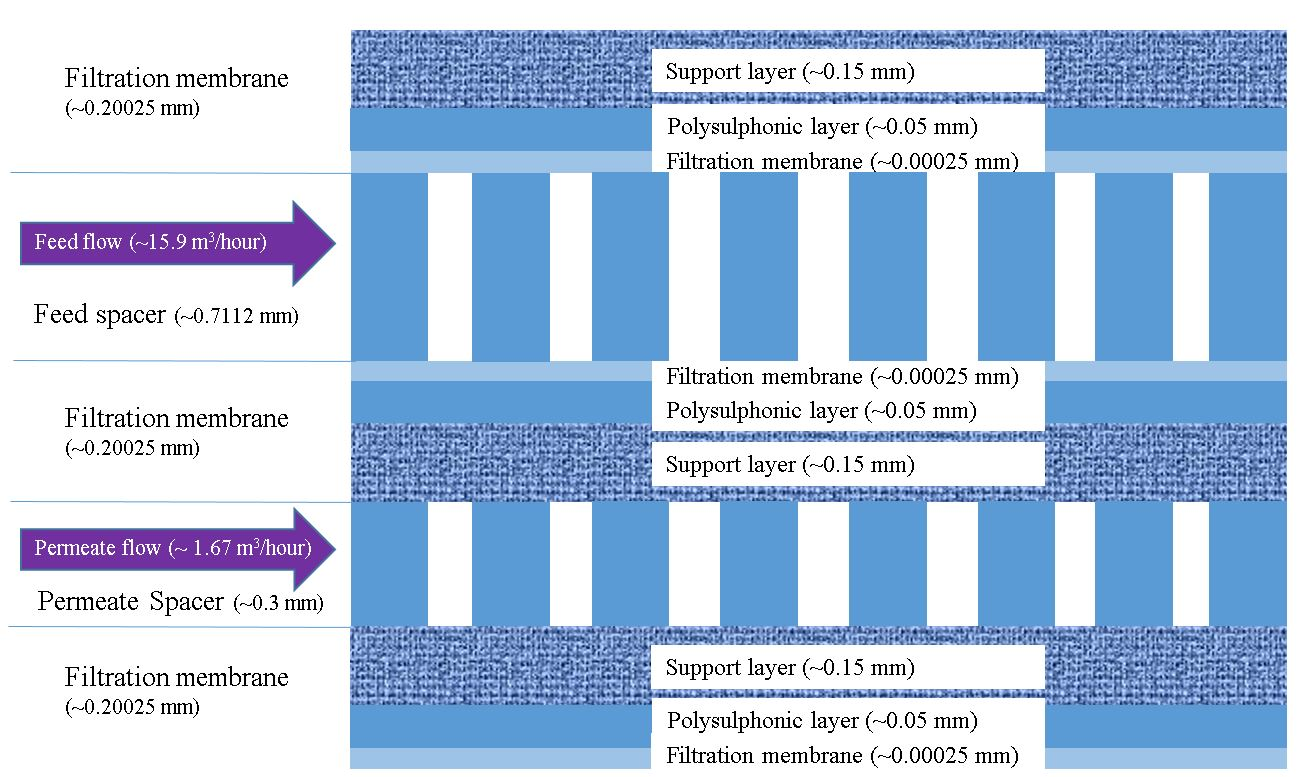
\includegraphics[width = \textwidth]{images/Introduction/membrane_schema.jpg}
    \caption{
        A cross-section of the RO polyamide filtration membrane \cite{Strubbe2018CalibrationFull-Scale}. The quantitative specifications are representative of the default values for our RO model, which are primarily based upon the DOW FILMTEC BW30-400 module.
    }
    \label{membrane_schema}
\end{figure}

\subsection{Scaling}
Scaling in Figure \ref{desalination_schema} is a geochemical phenomena that can occlude and tear the filtration membrane. The geochemical equilibria that result in scaling are difficult to experimentally study; hence, computational software that predict scaling have been developed \cite{Strubbe2018CalibrationFull-Scale}. These software, however, are expensive and/or not accessible via an API, which limits its accessibility and its ability to guide investigators through experimental design. We therefore developed a one-dimensional reactive transport model of desalination, which is sufficiently simple to be numerically encoded in PHREEQC. This PHREEQC expression of our model is the basis of our software, ROSSpy (Reverse Osmosis Scaling Software in Python), which is an intuitive and open-source API that meets identified needs of the RO community to predict brine and scaling from desalination systems. This project is detailed with validation and use cases in Chapter 2.

\begin{figure}
    \centering
    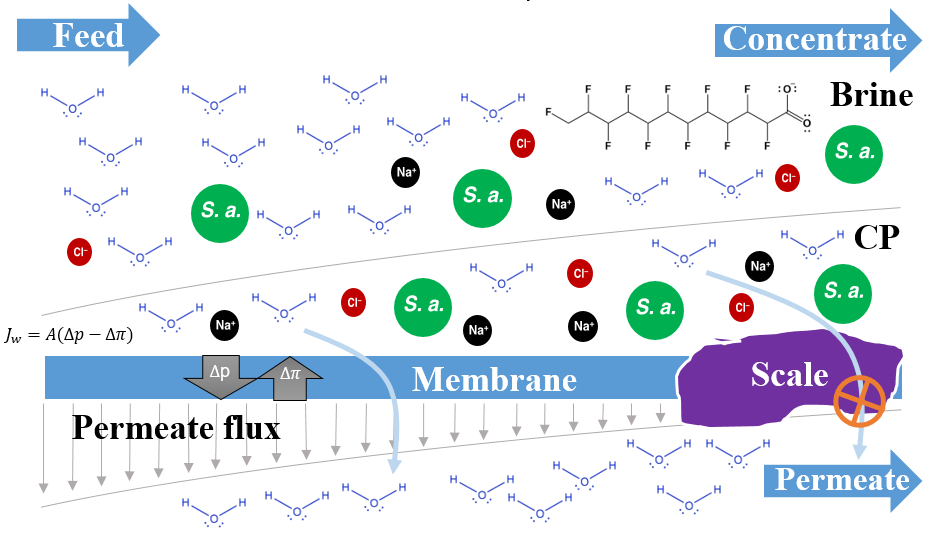
\includegraphics[width = \textwidth]{images/Introduction/desalination_schema_3.PNG}
    \caption{
        A cross-section of RO desalination, which depicts the geochemical environment and the physical hindrance of scaling upon the membrane surface.  Membrane flux decreases over the module distance as a function of the pressure difference between the applied pressure of the feed and the osmotic pressure between the filtered (permeate) water and brine (concentrate) solution.    
    }
    \label{desalination_schema}
\end{figure}

\subsection{Biofouling}
Biofouling is a microbial phenomena, where a surface is colonized and eventually biodegraded. Biocidal treatments can limit biofouling \cite{Kim2009BiocideOverview}, however, these treatments have substantial collateral effects of chemically degrading the filtration membrane \cite{Da-Silva-Correa2022TheReview} and possibly exhibiting off-target effects in the environment \cite{Martins2018Review:Ecosystems,Thomas2001AntifoulingEffects}. The design of benign anti-biofoulants \cite{Buckley2017DesignProducts} is therefore essential to improve the efficacy and sustainability of RO desalination. Innovation here \cite{Winters1983ControlDesalination} can be accelerated by computational tools that allow investigators to predict the effect of different chemical agents and biofilm conditions. We therefore developed the WCMpy (Whole Cell Model in Python) suite of packages to foster the development of such computational tools, which is detailed in Chapter 3. 

% The anti-biofoulant tributyltin oxide, for example, is applied in the coating of boat hulls, yet the chemical gradually leaches into the marine ecosystem where it acts as an immunological toxin to marine animals. An expanding social consciousness of anthropogenic pollution in nature and ultimately human toxification through biomagnification, is encouraging the development of highly specific anti-biofoulants that prevent or treat biofouling without off-target effects.

\section{Antimicrobial resistance}
The treatment of RO biofouling with antibiotics is intertwined with the AMR crisis, where AMR infections are projected to exceed cancer in annual deaths, and globally cost $10^{13}~USD$ in lost economic production, by the mid-21$^{st}$ century \cite{ONeill2014AntimicrobialNations}. The AMR crisis may be mitigated through the use of reactive oxygen species (ROSs), which non-selectively oxidize and kill pathogens while avoiding the mechanisms that result in AMR. ROSs, primarily singlet oxygen ($^1\Delta_g$), can be wielded on demand through photodynamic inactivation (PDI) by simply exposing a photosensitizer (PS) catalyst to incident light of the porper wavelength, which is illustrated in Figure \ref{PDI_workflow}. The innumerable possible combinations of PSs and undesirable microbial targets are unlikely to be completely explored with experiments before mid-century, since resource limitations restrain experimentation. We therefore developed the PDIpy module (Photodynamic Inactivation in Python) to rapidly predict PDI efficacy over a continuum of variable values, which can elucidate effective systems within the space of possible PDI technologies. This project is detailed in Chapter 4. 

\begin{figure}
    \centering
    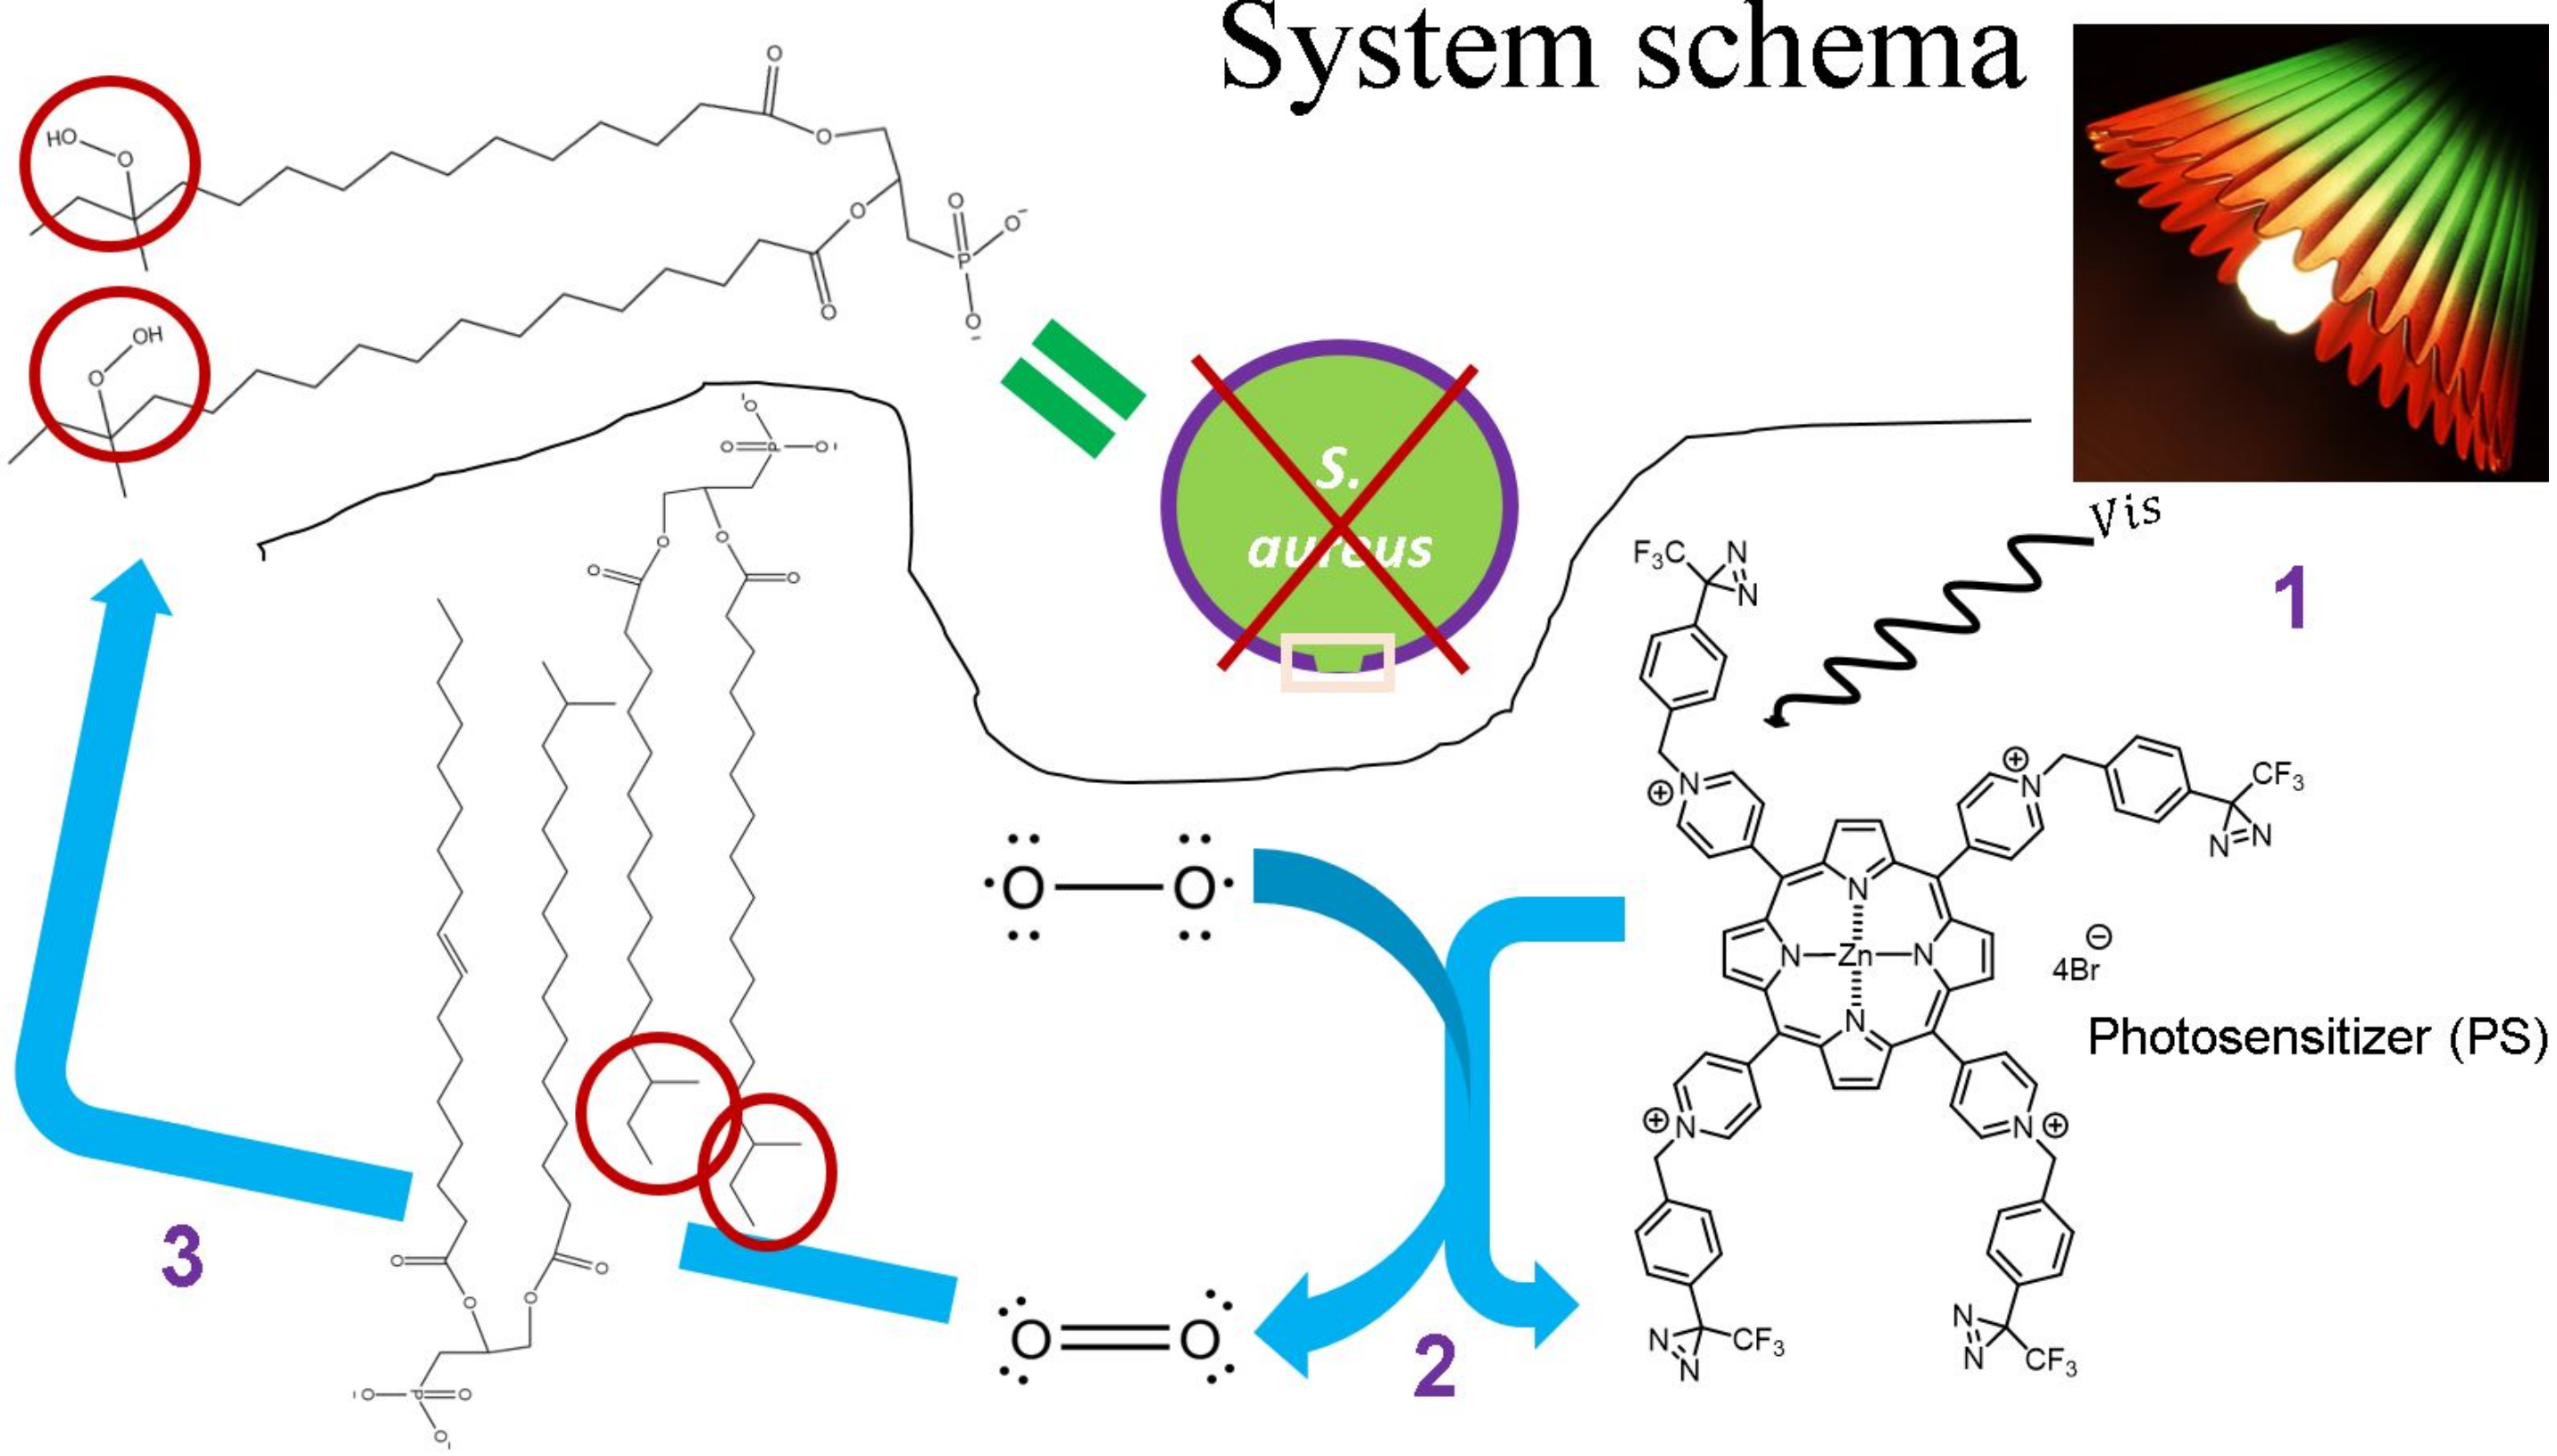
\includegraphics[width = \textwidth]{images/Introduction/PDI_workflow.png}
    \caption{
        A conceptualization of the PDI process: 1) incident light first strikes and excites a PS; 2) the excited PS catalyzes the generation of $\ce{^1O_2}$ from a ground-state oxygen; and 3) the $\ce{^3O_2}$ oxidizes a biological target to the point of cellular death.   
    }
    \label{PDI_workflow}
\end{figure}

\section{Thesis work}
All of the figures and tables in this Thesis are original. The Python modules that have been published in the PyPI (Python Package Index) repository, at least partially for the completion of this Thesis, are listed in Table \ref{downloads} with their respective quantity of PyPI downloads.

\begin{table}
    \centering
    \begin{tabular}{l|c|c|l}
        \textbf{Project} & \textbf{Module} & \textbf{PyPI~downloads} & \textbf{Total}\\
        \toprule
        \multirow{2}{2mm}{ROSSpy} & \href{https://github.com/freiburgermsu/ROSSpy}{ROSSpy} & 10,013 & \multirow{2}{2mm}{21,956}\\
         & \href{https://github.com/freiburgermsu/ChemW}{ChemW} & 11,943 & \\
         \hline
        \multirow{3}{2mm}{WCMpy} & \href{https://github.com/freiburgermsu/Codons}{Codons} & 4,316 & \multirow{3}{2mm}{5,662}\\
         & \href{https://github.com/freiburgermsu/BiGG_SABIO}{BiGG\_SABIO}  & 511 & \\
         & \href{https://github.com/freiburgermsu/dFBApy}{dFBApy} & 835 & \\
         \hline
        PDIpy & \href{https://github.com/freiburgermsu/PDIpy}{PDIpy} & 2,013 & 2,013\\
         \hline
         \textbf{Total} &  &  & \textbf{29,631} \\
         \bottomrule
    \end{tabular}
    \caption{
        The cumulative PyPI downloads according to PePy (\url{https://pepy.tech/}) -- per March 23th, 2022 -- for each of the modules and projects of this Thesis. The GitHub repositories for each module are hyperlinked with the respective module name. 
    }
    \label{downloads}
\end{table}


\section{Future}
The future aspirations for these projects are detailed in Chapter 5. The most notable far-term aspirations include the following: (1) amalgamate the WCMpy suite into a single module that simulates the biochemical effects of an anti-biofilm treatment; and (2) couple the mature module from (1) with the brine predictions from ROSSpy to comprehensively represent the effects of scaling and biofouling, and their interdependence \cite{Radu2014ASystems,Radu2010ModelingPassage}, from RO desalination. This may include the assessment of halophilic bacteria \cite{Bagheri2019ARuber} that could thrive in RO brine.